\setAuthor{Valter Kiisk}
\setRound{lahtine}
\setYear{2023}
\setNumber{G 5}
\setDifficulty{5}
\setTopic{TODO}

\prob{Elektriauto}
Gaafikul on kujutatud teatava elektriauto mootori kasuliku mehaanilise võimsuse sõltuvus kiirusest. Auto mass on $m=\SI{2200}{kg}$.\\
\osa Milline on suurim võimalik kiirendus?\\
\osa Minimaalselt kui kaua aega kulub 100 km tunnikiiruse saavutamiseks?\\
Õhutakistust ja rehvi libisemist teekattel võib ignoreerida.


\begin{figure}[h]
    \centering
    \vspace{-10pt}
    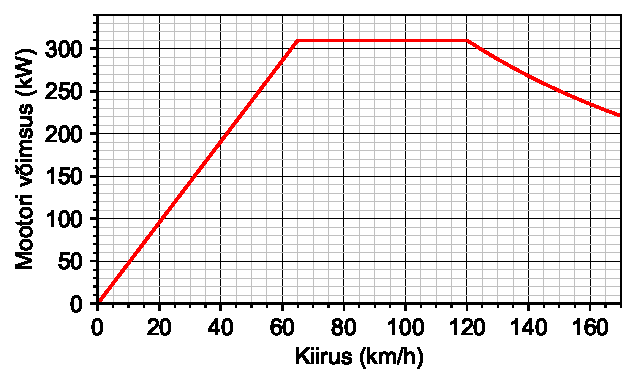
\includegraphics[width=0.75\linewidth]{2023-lahg-05-yl.pdf}
    \vspace{-35pt}
\end{figure}




\hint

\solu
\osa Autot kiirendav jõud avaldub võimsuse $P$ ja kiiruse $v$ kaudu: $F=P/v$. Graafikult on näha, et väikestel kiirustel $P$ kasvab võrdeliselt $v$-ga, nii et
\[
F=\frac{\SI{310}{\kilo\watt}}{\SI{65}{\kilo\meter\per\hour}}
\approx\frac{\SI{310000}{\watt}}{\SI{18}{\meter\per\second}}\approx\SI{17200}{\newton}
\]
Suurematel kiirustel $P$ jääb konstandiks või väheneb, seega maksimaalne veojõud ongi \SI{17200}{N} ja vastav kiirendus $a=F/m=\SI{7.8}{\meter\per\second\squared}$.

\osa Kuni kiiruseni $v_1=\SI{65}{\kilo\meter\per\hour}=\SI{18}{\meter\per\second}$ kulgeb auto ühtlase kiirendusega $a=\SI{7.8}{\meter\per\second\squared}$. Selle kiiruse saavutamiseks kulub aega
\[
t_1=\frac{v_1}{a}= \frac{\SI{18}{\meter\per\second}}{\SI{7.8}{\meter\per\second\squared}} \approx \SI{2.3}{s}.
\]
Suurematel kiirustel (kuni $v_2=\SI{100}{\kilo\meter\per\hour}$) mootori võimsus on konstant ($P=\SI{310}{\kilo\watt}$), seega kiirendus ajas muutub. Kiirenduse asemel on nüüd mugavam opereerida kineetilise energiaga. Kogu kasulik võimsus läheb auto kineetilise energia suurendamiseks, seega
\[
Pt_2=\frac{mv_2^2}{2} - \frac{mv_1^2}{2},
\]
millest
\[
t_2=\frac{m}{2P}(v_2^2-v_1^2)\approx \frac{\SI{2200}{\kilo\gram}}{2\cdot \SI{310000}{\watt}}\left[(\SI{28}{\meter\per\second})^2 - (\SI{18}{\meter\per\second})^2 \right]\approx \SI{1.6}{s}.
\]
Seega aega kulub kokku $t_1+t_2=\SI{3.9}{s}$.
\probend